\documentclass[11pt,a4paper]{article}
\usepackage[T1]{fontenc}
\usepackage[utf8]{inputenc}
\usepackage{lmodern}
\usepackage{microtype}
\usepackage[margin=27mm,headheight=15pt]{geometry}
\usepackage{amsmath,amssymb,amsthm,mathtools,bm,mathrsfs}
\usepackage{booktabs,array,longtable}
\usepackage{graphicx,xcolor}
\usepackage{float}
\usepackage{enumitem}
\usepackage{fancyhdr}
\usepackage{listings}
\usepackage[numbers]{natbib}
\usepackage{xurl}
\usepackage{hyperref}
\usepackage[nameinlink,capitalize,noabbrev]{cleveref}
\definecolor{ink}{HTML}{16354A}
\definecolor{accent}{HTML}{167B86}
\definecolor{pale}{HTML}{F0F5F7}
\hypersetup{colorlinks=true,linkcolor=ink,citecolor=accent,urlcolor=accent,
  pdftitle={Sharp and Computable Corrections for Nonuniform Coupon Collection},
  pdfauthor={Research prepared for Vladimir Reshetnikov}}
\pagestyle{fancy}
\fancyhf{}
\fancyhead[L]{\small\textsc{Certified coupon collection}}
\fancyhead[R]{\small Research manuscript}
\fancyfoot[C]{\thepage}
\renewcommand{\headrulewidth}{0.3pt}
\setlength{\emergencystretch}{2em}
\setlist[itemize]{topsep=4pt,itemsep=3pt,parsep=0pt}
\setlist[enumerate]{topsep=4pt,itemsep=3pt,parsep=0pt}
\lstset{basicstyle=\ttfamily\small,breaklines=true,frame=single,
  rulecolor=\color{pale},backgroundcolor=\color{pale},columns=fullflexible,
  keepspaces=true,showstringspaces=false}
\newtheorem{theorem}{Theorem}[section]
\newtheorem{lemma}[theorem]{Lemma}
\newtheorem{proposition}[theorem]{Proposition}
\newtheorem{corollary}[theorem]{Corollary}
\theoremstyle{definition}
\newtheorem{definition}[theorem]{Definition}
\newtheorem{remark}[theorem]{Remark}
\newcommand{\E}{\mathbb E}
\newcommand{\Prb}{\mathbb P}
\newcommand{\N}{\mathbb N}
\newcommand{\R}{\mathbb R}
\newcommand{\dd}{\,\mathrm d}
\newcommand{\coeff}[2]{[#1^{#2}]}
\newcommand{\bigO}{\mathcal O}
\newcommand{\Kopt}{\mathcal K}
\DeclareMathOperator{\Var}{Var}
\DeclareMathOperator{\supp}{supp}
\graphicspath{{../figures/}}

\begin{document}
\begin{titlepage}
\vspace*{13mm}
{\color{accent}\large\textsc{Probability, asymptotic analysis, and certified computation}\par}
\vspace{12mm}
{\color{ink}\huge\bfseries Sharp and Computable Corrections\\[4pt]
for Nonuniform Coupon Collection\par}
\vspace{8mm}
{\Large A positive remainder bound, optimal kernel constants,\\
and a deterministic algorithm with probability enclosures\par}
\vspace{12mm}
{\large Research prepared for Vladimir Reshetnikov\par}
\vspace{3mm}
{8 October 2026\par}
\vspace{12mm}
\begin{abstract}
The probability of observing every category in a fixed number of independent
samples is easy to approximate after Poissonization, but a numerical
approximation is substantially more useful when accompanied by a computable
error bound. We refine a recent Taylor-remainder lemma of Hwang, Li, and
Zacharovas for the kernel $(1-x)^m e^{mx}$. A change of variable with
nonnegative Taylor coefficients produces an explicit pointwise bound that
is smaller throughout the original domain. Its integration yields a positive
moment certificate for arbitrary coupon probabilities.

For truncation before degree $2s$, we determine the optimal scalar remainder
constant through its second asymptotic term:
\[
 \Kopt_{m,s}=\frac{m^s}{2^s s!}
 \left(1+\frac{s(-2s^2+5s+1)}{9m}+\bigO_s(m^{-2})\right).
\]
The maximizing argument is uniquely defined for sufficiently large $m$ and
equals $2s(s+1)/(3m)+\bigO_s(m^{-2})$. Both quantities admit convergent
expansions in $1/m$ near infinity at each fixed order. The positive moment
certificate is asymptotically attained by a rare-coupon family.

All derivatives and moments needed by the certificate are computed by
truncated products in $\bigO(ns^2)$ arithmetic operations, after an
order-dependent setup. An Arb implementation encloses both truncation and
rounding errors. We also give explicit bounds uniform over every probability
vector in the region $\sum_i e^{-mp_i}\le L$, recover the sharp scale
$(\log n/n)^s$, and provide reproducible numerical checks. The
Poisson--Charlier expansion itself is classical; the research contribution
is the refined remainder analysis and its constructive, certified use.
\end{abstract}
\vfill
{\small\color{ink}Complete proofs and executable verification accompany this
manuscript. The precise comparison with prior work is stated in
\cref{sec:position}; the asymptotic results keep $s$ fixed.}
\end{titlepage}

\tableofcontents
\newpage

\section{The problem and the result}\label{sec:introduction}

Suppose that each independent observation belongs to one of $n$ categories,
with known probabilities $p_1,\ldots,p_n$. How likely is it that all
categories have appeared after $m$ observations? This is the nonuniform
coupon collector problem. It is also a finite occupancy question: place
$m$ independent balls into $n$ boxes, choosing box $i$ with probability
$p_i$, and ask whether every box is occupied.

Write $T$ for the first time at which every category has appeared, and put
$P_m=\Prb(T\le m)$. The input assumptions throughout are
\begin{equation}\label{eq:domain}
 n\ge1,\qquad p_i\ge0,\qquad \sum_{i=1}^n p_i=1,
 \qquad m\in\N,\quad m\ge1.
\end{equation}
Zero probabilities and the condition $m<n$ are allowed. They make $P_m=0$,
but allowing them in the theorems is useful for checking boundary cases.

If the number of observations is instead Poisson with mean $t$, the box
counts are independent Poisson variables. The resulting coverage probability
is the elementary product
\begin{equation}\label{eq:Fintro}
 F(t)=\prod_{i=1}^n(1-e^{-tp_i}).
\end{equation}
Replacing the fixed sample size by a Poisson sample size is called
\emph{Poissonization}; recovering fixed-sample information is
\emph{depoissonization}. A product such as \eqref{eq:Fintro} can be evaluated
with one pass over the probabilities. The challenge is to retain this
computational simplicity while controlling the error at a fixed sample size.

\subsection{What is proved here}

The central finite result is the interval
\begin{equation}\label{eq:introinterval}
 P_m\in[A_s(m)-R_s(m),\,A_s(m)+R_s(m)]\cap[0,1],
\end{equation}
where $A_s$ is a classical Poisson--Charlier approximation and $R_s$ is an
explicit positive expression. It applies to every input in
\eqref{eq:domain}. It does not require comparable probabilities, a limit
distribution, or a large sample size. Those assumptions enter only when
describing how small the interval becomes asymptotically.

There are three complementary conclusions.
\begin{enumerate}
\item \textbf{A stronger finite bound.} The scalar inequality underlying
\eqref{eq:introinterval} improves an explicitly identified remainder lemma
on its full domain. It leads to a certificate involving moments through
order $3s$, all computed without enumerating subsets.
\item \textbf{Optimal constants.} The best scalar constant has an explicit
two-term asymptotic expansion. A genuine coupon-collector family attains
the leading constant in the positive moment certificate.
\item \textbf{An implementable calculation.} For each fixed $s$, the
arithmetic work grows linearly with $n$. The supplied interval-arithmetic
program returns a probability enclosure, and separate exact calculations
check the implementation on small instances.
\end{enumerate}

\subsection{Position relative to the literature}\label{sec:position}

Classical analytic depoissonization already supplies systematic expansions
in derivatives of the Poisson transform \cite{JacquetSz1998}. High-order
approximations for uniform coupon collection are also established
\cite{Posfai2010}. Recent elementary work gives explicit remainders using
finite differences \cite{Zacharovasv2}. Consequently, the expansion and
the existence of fixed-order asymptotic corrections are prior results.

The closest pointwise comparison is Lemma~5.3, equation~(46), of the May
2026 preprint of Hwang, Li, and Zacharovas \cite{HLZ2026}. With the
variables renamed as in this paper, it bounds a Taylor remainder by
\begin{equation}\label{eq:HLZ}
 \left|(1-x)^m e^{mx}-Q_{m,s}(x)\right|
 \le 2s\,4^s m^s x^{2s},\qquad 0\le x\le1,
\end{equation}
where $Q_{m,s}$ is the Taylor polynomial through degree $2s-1$.
\Cref{thm:scalar} replaces the coefficient by a smaller explicit polynomial
in $x$. For $s=1$, their earlier Lemma~2.1 has the better bound $mx^2$;
our coefficient is $m(1+x)/2$, which improves that comparison for
$0<x<1$ as well. We compare with the stated lemmas, rather than claim a
general improvement of every result in those papers.

The supplied repository \cite{OpenAIMath2026} motivated a search for a
quantitative theorem with an independently checkable proof and reusable
computational artifacts. Its approximate-counting families 113--115
suggested the guiding question: can a combinatorial probability be
approximated efficiently while retaining an explicit error guarantee?
All mathematical inputs used below are proved
in the manuscript or attributed to the established literature; the
repository's larger conjecture-resolution claims are not dependencies of
our proofs. The snapshot inspected was commit
\texttt{fd4aeeb2ee4fc729c18d98444fed42fd0529eeeb}.

\subsection{Scope of the claims}

The result is a concrete strengthening of an existing quantitative lemma,
together with sharp asymptotic analysis of its optimal constant. It does
not resolve a longstanding major open conjecture. The literature review
identified the overlap above; it cannot establish that every variant of
the remainder estimate is absent from all previous publications.

The certificate controls \emph{absolute} error. It can be uninformative
early in the collection process, and it does not automatically give small
relative error when $P_m$ is extremely small. All asymptotic expansions in
the truncation order keep $s$ fixed. The operation count is an arithmetic
count with exponential evaluations, not a theorem about bit complexity.
These distinctions are part of the mathematical statements, not exceptions
to them.

\section{Exact identities and notation}\label{sec:identities}

For $A\subseteq[n]$, let $p_A=\sum_{i\in A}p_i$. The event that every
category in $A$ is missing after $m$ observations has probability
$(1-p_A)^m$. Inclusion--exclusion therefore gives
\begin{equation}\label{eq:IE}
 P_m=\sum_{A\subseteq[n]}(-1)^{|A|}(1-p_A)^m.
\end{equation}
Expanding \eqref{eq:Fintro} gives the corresponding exponential sum:
\begin{equation}\label{eq:Fsum}
 F(t)=\sum_{A\subseteq[n]}(-1)^{|A|}e^{-tp_A}.
\end{equation}
These formulas show directly that
$F(t)=e^{-t}\sum_{m\ge0}P_m t^m/m!$ for $t\ge0$, with the natural
convention $P_0=0$. They also avoid needing an independence argument for
Poisson splitting in the proofs that follow.

Define the unsigned subset moments
\begin{equation}\label{eq:moments}
 M_k(t)=\sum_{A\subseteq[n]}p_A^k e^{-tp_A},\qquad k\ge1.
\end{equation}
The term $A=\varnothing$ is zero. The moments are nonnegative and satisfy
\begin{equation}\label{eq:momentmonotone}
 M_{k+1}(t)\le M_k(t),\qquad k\ge1,
\end{equation}
because $0\le p_A\le1$. In contrast,
\begin{equation}\label{eq:Fderiv}
 (-1)^kF^{(k)}(t)
   =\sum_A(-1)^{|A|}p_A^k e^{-tp_A}
\end{equation}
can have either sign. The unsigned moments preserve a rigorous error bound
when the inclusion--exclusion terms cancel.

\begin{remark}[A larger class]\label{rem:mixtures}
Let $\mu$ be a finite signed or complex measure on $[0,1]$, and define
\[
 a_m=\int(1-x)^m\dd\mu(x),\qquad
 f(t)=\int e^{-tx}\dd\mu(x),\qquad
 M_k^{\mu}(t)=\int x^k e^{-tx}\dd|\mu|(x).
\]
The same proofs apply with these definitions. For coupon collection,
$\mu=\sum_A(-1)^{|A|}\delta_{p_A}$. If distinct subsets have the same
total probability, opposite signs may cancel in $\mu$. The explicit
$M_k$ in \eqref{eq:moments} is still a valid positive majorant for
$M_k^{\mu}$ and is easier to compute by products.
\end{remark}

\section{A positive-coefficient remainder bound}\label{sec:scalar}

\subsection{The classical Taylor coefficients}

For an integer $m\ge1$, define
\begin{equation}\label{eq:kernel}
 E_m(x)=(1-x)^m e^{mx}=\sum_{k\ge0}c_k(m)x^k,
 \qquad Q_{m,s}(x)=\sum_{k=0}^{2s-1}c_k(m)x^k.
\end{equation}
The function $E_m$ is entire. Logarithmic differentiation near the origin
gives
\begin{equation}\label{eq:crecurrence}
 c_0(m)=1,\quad c_1(m)=0,\qquad
 k c_k(m)=-m\sum_{j=0}^{k-2}c_j(m)\quad(k\ge2).
\end{equation}
Keeping prefix sums evaluates this recurrence in linear arithmetic work
in the number of coefficients. For example,
\begin{align}\label{eq:firstc}
 c_2&=-\frac m2,&c_3&=-\frac m3,&
 c_4&=\frac{m^2}{8}-\frac m4,&
 c_5&=\frac{m^2}{6}-\frac m5.\nonumber
\end{align}
We suppress the argument $m$ in short formulas.

\begin{lemma}[Degree and first omitted coefficient]\label{lem:degree}
For fixed $k$, $c_k(m)$ is a polynomial in $m$ of degree at most
$\lfloor k/2\rfloor$. In particular,
\begin{equation}\label{eq:leadingc}
 c_{2s}(m)=\frac{(-1)^s m^s}{2^s s!}
             +\bigO_s(m^{s-1}).
\end{equation}
\end{lemma}
\begin{proof}
For $|x|<1$,
\[
 E_m(x)=\exp\left(-m\sum_{j\ge2}\frac{x^j}{j}\right).
\]
Every factor contributing a power of $m$ has degree at least two in $x$.
The coefficient of $m^s x^{2s}$ can therefore only come from $s$ copies of
$-mx^2/2$, proving both statements.
\end{proof}

\subsection{A change of variable}

Put
\begin{equation}\label{eq:d}
 d(x)=1-(1-x)e^x=\sum_{k\ge2}\frac{k-1}{k!}x^k.
\end{equation}
All coefficients are nonnegative, $d(1)=1$, and the coefficient of $x^2$
is $1/2$. It follows that, on the full interval $0\le x\le1$,
\begin{equation}\label{eq:dmajorant}
 0\le d(x)\le\frac{x^2}{2}(1+x)\le x^2.
\end{equation}
Indeed, all terms of degree at least three have total coefficient $1/2$
and are bounded by that coefficient times $x^3$.

For $1\le j<s$, define the rational constants
\begin{equation}\label{eq:theta}
 \theta_{j,2s}
   =1-\sum_{k=0}^{2s-1}[x^k]d(x)^j,
 \qquad
 B_{m,s}=\sum_{j=1}^{s-1}\binom mj\theta_{j,2s}.
\end{equation}
The sum defining $B_{m,1}$ is empty and equals zero. Since the
coefficients of $d^j$ are nonnegative and sum to $d(1)^j=1$,
\begin{equation}\label{eq:theta01}
 0\le\theta_{j,2s}\le1.
\end{equation}
We use the convention $\binom mj=0$ for $j>m$.

\begin{theorem}[Pointwise finite refinement]\label{thm:scalar}
For all integers $m,s\ge1$ and all $0\le x\le1$,
\begin{equation}\label{eq:scalarbound}
 |E_m(x)-Q_{m,s}(x)|
 \le x^{2s}\left(
 B_{m,s}+\frac{\binom ms}{2^s}(1+x)^s\right).
\end{equation}
\end{theorem}
\begin{proof}
First assume $m\ge s$. Taylor's theorem for $(1-y)^m$ on $0\le y\le1$
gives
\begin{equation}\label{eq:binomialremainder}
 \left|(1-y)^m-\sum_{j=0}^{s-1}(-1)^j\binom mj y^j\right|
 \le\binom ms y^s.
\end{equation}
The absolute value of the $s$th derivative is at most
$s!\binom ms$ on this interval. If $m<s$, the finite sum already equals
$(1-y)^m$, and the same inequality holds with a zero right-hand side.

Substitute $y=d(x)$. The identity $1-d(x)=(1-x)e^x$ gives
$(1-d(x))^m=E_m(x)$. Every omitted power $d(x)^j$ with $j\ge s$
starts at degree at least $2s$. Thus the Taylor polynomial through degree
$2s-1$ of the finite sum in \eqref{eq:binomialremainder} is exactly
$Q_{m,s}$.

For each $1\le j<s$, the discarded coefficient tail satisfies
\[
 0\le d(x)^j-\sum_{k=0}^{2s-1}([x^k]d(x)^j)x^k
 \le\theta_{j,2s}x^{2s}.
\]
This uses $x^k\le x^{2s}$ for $k\ge2s$ and the nonnegative coefficients.
Adding the finite Taylor-tail errors and the binomial remainder gives
\[
 |E_m(x)-Q_{m,s}(x)|
 \le B_{m,s}x^{2s}+\binom ms d(x)^s.
\]
Now apply \eqref{eq:dmajorant}. Every step holds at $x=1$ as well as in
the interior, so there is no endpoint exception.
\end{proof}

\begin{corollary}[Direct comparison with the prior lemma]\label{cor:comparison}
The coefficient in \eqref{eq:scalarbound} satisfies
\begin{equation}\label{eq:coarsecoef}
 B_{m,s}+\frac{\binom ms}{2^s}(1+x)^s
 \le\sum_{j=1}^s\binom mj
 \le m^s\sum_{j=1}^s\frac1{j!}
 <(e-1)m^s.
\end{equation}
In particular, \eqref{eq:scalarbound} is a pointwise refinement of
\eqref{eq:HLZ}, with a strictly smaller upper-bound function for $x>0$.
For $s=1$ it is
\begin{equation}\label{eq:s1scalar}
 |E_m(x)-1|\le\frac m2x^2(1+x).
\end{equation}
\end{corollary}
\begin{proof}
Use \eqref{eq:theta01} and $(1+x)^s\le2^s$. Then use
$\binom mj\le m^j/j!\le m^s/j!$ for $j\le s$ and $m\ge1$.
\end{proof}

\section{The certified coupon probability}\label{sec:certificate}

Define the approximant and its error radius by
\begin{equation}\label{eq:approx}
 A_s(m)=\sum_{k=0}^{2s-1}(-1)^k c_k(m)F^{(k)}(m),
\end{equation}
and
\begin{equation}\label{eq:radius}
 \boxed{\quad
 R_s(m)=B_{m,s}M_{2s}(m)
 +\frac{\binom ms}{2^s}
     \sum_{\ell=0}^s\binom s\ell M_{2s+\ell}(m).
 \quad}
\end{equation}
Every contribution to \eqref{eq:radius} is nonnegative.

\begin{theorem}[Finite probability enclosure]\label{thm:coupon}
Under \eqref{eq:domain}, for every integer $s\ge1$,
\begin{equation}\label{eq:certtheorem}
 |P_m-A_s(m)|\le R_s(m).
\end{equation}
The same assertion holds in \cref{rem:mixtures}, with total-variation
moments in place of the unsigned subset moments.
\end{theorem}
\begin{proof}
Multiply \eqref{eq:scalarbound} by $e^{-mx}$ and set $x=p_A$.
Subtract the signed sums in \eqref{eq:IE} and \eqref{eq:Fderiv}.
The triangle inequality bounds the difference by
\[
 \sum_A e^{-mp_A}p_A^{2s}
 \left(B_{m,s}+\frac{\binom ms}{2^s}(1+p_A)^s\right).
\]
Expanding $(1+p_A)^s$ gives precisely \eqref{eq:radius}. Integration
against $|\mu|$ proves the more general version.
\end{proof}

\subsection{The first useful orders}

All derivatives and moments in the following formulas are evaluated at
$t=m$. At order one,
\begin{equation}\label{eq:order1}
 A_1=F,\qquad R_1=\frac m2(M_2+M_3).
\end{equation}
At order two,
\begin{align}
 A_2&=F-\frac m2 F''+\frac m3F''',\label{eq:order2a}\\
 R_2&=\frac m6M_4+\frac{m(m-1)}8(M_4+2M_5+M_6).
 \label{eq:order2r}
\end{align}
The cubic derivative in \eqref{eq:order2a} is included deliberately:
the approximation is the full Taylor truncation through degree three.
At order three,
\begin{align}
 A_3={}&F-\frac m2F''+\frac m3F'''
       +\left(\frac{m^2}8-\frac m4\right)F^{(4)}
       +\left(\frac m5-\frac{m^2}6\right)F^{(5)},
       \label{eq:order3a}\\
 B_{m,3}={}&\frac m{120}+\frac5{12}\binom m2,\nonumber\\
 R_3={}&B_{m,3}M_6+\frac{\binom m3}{8}
               (M_6+3M_7+3M_8+M_9).
       \label{eq:order3r}
\end{align}
For example, $\theta_{1,4}=1/6$,
$\theta_{1,6}=1/120$, and $\theta_{2,6}=5/12$ follow from
\eqref{eq:d}. The supplied code computes these quantities as exact
rationals rather than decimal approximations.

\subsection{Comparison of the integrated bounds}

The monotonicity \eqref{eq:momentmonotone} gives
\begin{equation}\label{eq:coarseradius}
 R_s(m)\le
 \left(B_{m,s}+\binom ms\right)M_{2s}(m)
 \le\left(\sum_{j=1}^s\binom mj\right)M_{2s}(m).
\end{equation}
Thus retaining the additional moments never worsens the corresponding
coarse positive-moment bound. Direct integration of \eqref{eq:HLZ}
would instead give $2s4^s m^sM_{2s}(m)$.

For completeness, the general finite-difference theorem of
\cite[Theorem~1.2, version~2]{Zacharovasv2} gives a remainder
$33m^s\mathcal E_{2s}(m)$ for $m\ge2$. In the measure setting,
\[
 \Delta^{2s}a_j=\int x^{2s}(1-x)^j\dd\mu(x),\qquad
 \mathcal E_{2s}(m)
 =e^{-m}\sum_{j\ge0}\frac{m^j}{j!}|\Delta^{2s}a_j|
 \le M_{2s}^{\mu}(m).
\]
Our radius is smaller than its computable unsigned-majorant specialization
$33m^sM_{2s}(m)$. The original seminorm may exploit cancellation, so this
is not a dominance claim against $33m^s\mathcal E_{2s}(m)$ itself.

\section{The optimal scalar constant}\label{sec:optimal}

\subsection{Its leading term is best possible}

\begin{definition}
The optimal scalar coefficient for the truncation at order $s$ is
\begin{equation}\label{eq:Kdef}
 \Kopt_{m,s}=\sup_{0<x\le1}
      \frac{|E_m(x)-Q_{m,s}(x)|}{x^{2s}}.
\end{equation}
The quotient has its removable value $|c_{2s}(m)|$ at $x=0$.
\end{definition}

\begin{theorem}[Optimal leading coefficient]\label{thm:optimalfirst}
For every fixed integer $s\ge1$,
\begin{equation}\label{eq:Kleading}
 \Kopt_{m,s}\sim\frac{m^s}{2^s s!}\qquad(m\longrightarrow\infty).
\end{equation}
\end{theorem}
\begin{proof}
Taking $x\downarrow0$ in \eqref{eq:Kdef} and applying
\cref{lem:degree} gives the required lower limit.

For the upper limit, fix $\delta\in(0,1)$. On $0<x\le\delta$,
\cref{thm:scalar} gives
\[
 \frac{|E_m(x)-Q_{m,s}(x)|}{m^s x^{2s}}
 \le\frac{B_{m,s}}{m^s}
    +\frac{\binom ms}{2^s m^s}(1+\delta)^s.
\]
Here $B_{m,s}=\bigO_s(m^{s-1})$ and
$\binom ms/m^s\to1/s!$. On $\delta\le x\le1$, the kernel is
between zero and one, while all retained coefficients have degree at most
$s-1$ in $m$. Hence the supremum of the normalized quotient over that
subinterval is $\bigO_{s,\delta}(m^{-1})$. Send $m$ to infinity and
then send $\delta$ to zero.
\end{proof}

The supremum of the explicit polynomial envelope in
\eqref{eq:scalarbound} is not asymptotically the same as
$\Kopt_{m,s}$. The split in this proof keeps the additional information
that the actual Taylor polynomial is small relative to $m^s$ when $x$
stays away from zero.

\subsection{A second term and a unique worst argument}

\begin{theorem}[Sharp second-order asymptotics]\label{thm:optimalsecond}
Fix $s\ge1$. For all sufficiently large integers $m$, the quotient in
\eqref{eq:Kdef} attains its global maximum at a unique point
$x_{m,s}\in(0,1)$. Moreover,
\begin{align}
 x_{m,s}&=\frac{2s(s+1)}{3m}+\bigO_s(m^{-2}),\label{eq:xmax}\\
 \Kopt_{m,s}&=\frac{m^s}{2^s s!}
 \left(1+\frac{s(-2s^2+5s+1)}{9m}
            +\bigO_s(m^{-2})\right).\label{eq:Ksecond}
\end{align}
More strongly, $m x_{m,s}$ and $m^{-s}\Kopt_{m,s}$ are restrictions of
real-analytic functions of $1/m$ near zero. Their expansions in $1/m$
therefore converge for sufficiently large $m$ at each fixed $s$.
\end{theorem}

\begin{proof}
We first establish global localization, then use a local analytic maximum.
Put $\varepsilon=m^{-1/2}$ and $y=x/\varepsilon$. In the physical
range $0\le y<1/\varepsilon$, set
\begin{equation}\label{eq:fscaled}
 f_\varepsilon(y)=
 \exp\left(\varepsilon^{-2}
          [\log(1-\varepsilon y)+\varepsilon y]\right).
\end{equation}
Its value at $y=1/\varepsilon$ is zero. At $\varepsilon=0$, define
$f_0(y)=e^{-y^2/2}$. On every fixed compact interval, the series
\begin{equation}\label{eq:scaledlog}
 \log f_\varepsilon(y)
   =-\frac{y^2}{2}-\sum_{k\ge3}\frac{\varepsilon^{k-2}y^k}{k}
\end{equation}
and any fixed number of its derivatives converge uniformly when
$|\varepsilon y|\le1/2$.

Let $\mathsf T_{2s-1}$ denote Taylor truncation in $y$, and define the
signed normalized remainder
\begin{equation}\label{eq:Hscaled}
 H_\varepsilon(y)=(-1)^s
 \frac{f_\varepsilon(y)-\mathsf T_{2s-1}f_\varepsilon(y)}{y^{2s}}.
\end{equation}
The value at $y=0$ is removable. The integral Taylor-remainder formula
shows that $H_\varepsilon\to H_0$ in $C^2$ on every fixed compact
interval. Explicitly,
\begin{equation}\label{eq:Hgaussian}
 H_0(y)=\frac1{2^s(s-1)!}
    \int_0^1(1-t)^{s-1}e^{-ty^2/2}\dd t.
\end{equation}
This is positive and strictly decreasing for $y>0$, with
$H_0(0)=\kappa_s:=1/(2^ss!)$.

We also need control on intervals growing with $m$. Since
$0\le f_\varepsilon(y)\le e^{-y^2/2}$, and the scaled Taylor
coefficients satisfy
\[
 c_{2j}(m)m^{-j}=\bigO_s(1),\qquad
 c_{2j+1}(m)m^{-j-1/2}=\bigO_s(\varepsilon),
\]
there is a constant $C_s$ such that for $R\ge1$ and
$R\le y\le1/\varepsilon$,
\begin{equation}\label{eq:Htail}
 |H_\varepsilon(y)|\le\frac{C_s}{R^2}
                                  +\frac{C_s\varepsilon}{R}.
\end{equation}
For the even terms the largest retained degree is $2s-2$; for the odd
terms it is $2s-1$. These two facts give the two powers of $R$ in
\eqref{eq:Htail}. The constant term and the kernel are covered by the
same estimate.

Fix a small $\delta>0$. Choose a large fixed $R$ so that the tail bound
is smaller than $\kappa_s/2$. On $[\delta,R]$, the strict decrease in
\eqref{eq:Hgaussian} and uniform convergence give a fixed gap below
$\kappa_s$. Since $H_\varepsilon(0)\to\kappa_s$, every global
maximizer of $|H_\varepsilon|$ eventually lies in $[0,\delta]$.

The series \eqref{eq:scaledlog} is jointly analytic near
$(\varepsilon,y)=(0,0)$. Removing the Taylor terms and dividing by
$y^{2s}$ preserves that analyticity. There is also the symmetry
\begin{equation}\label{eq:Hsymmetry}
 H_{-\varepsilon}(-y)=H_\varepsilon(y).
\end{equation}
The first terms of the local expansion are
\begin{equation}\label{eq:Hlocal}
 H_\varepsilon(y)=\kappa_s-D_s\varepsilon^2
                      +U_s\varepsilon y-V_s y^2
                      +\bigO_s((|\varepsilon|+|y|)^4),
\end{equation}
where
\begin{align*}
 U_s&=\frac1{3\,2^{s-1}(s-1)!},&
 V_s&=\frac1{2^{s+1}(s+1)!},\\
 D_s&=\kappa_s\frac{s(s-1)(4s+1)}9.
\end{align*}
To obtain $D_s$, the next coefficient of $c_{2s}$ has either one
part of size four and $s-2$ parts of size two, or two parts of size
three and $s-3$ parts of size two in the exponential in
\cref{lem:degree}. An impossible part pattern contributes zero.
The coefficient $U_s$ comes from one part of size three in
$c_{2s+1}$; $-V_s$ comes from the leading term of $c_{2s+2}$.
The symmetry \eqref{eq:Hsymmetry} rules out odd total degree in
\eqref{eq:Hlocal}.

Since $H_0''(0)=-2V_s<0$, take $\delta$ small enough that $H_0$ is
strictly concave and positive on $[0,\delta]$. The $C^2$ convergence
makes the same true for $H_\varepsilon$ at small positive
$\varepsilon$. Moreover,
$H_\varepsilon'(0)=U_s\varepsilon+\bigO_s(\varepsilon^3)>0$ and
$H_\varepsilon'(\delta)<0$. There is a unique maximum in the
interval, and global localization makes it the unique global maximum of
the absolute quotient.

The analytic implicit-function theorem applied to
$\partial_y H_\varepsilon(y)=0$ gives an analytic critical point
$y(\varepsilon)$ near zero. By symmetry and uniqueness it is odd.
Therefore
\[
 y(\varepsilon)=\frac{U_s}{2V_s}\varepsilon
                      +\bigO_s(\varepsilon^3)
 =\frac{2s(s+1)}3\varepsilon+\bigO_s(\varepsilon^3).
\]
Substituting in \eqref{eq:Hlocal} gives
\[
 H_\varepsilon(y(\varepsilon))
 =\kappa_s+\left(\frac{U_s^2}{4V_s}-D_s\right)\varepsilon^2
                  +\bigO_s(\varepsilon^4).
\]
The quotient of the parenthesized coefficient by $\kappa_s$ is
$s(-2s^2+5s+1)/9$. Finally,
$x_{m,s}=\varepsilon y(\varepsilon)$ and
$\Kopt_{m,s}/m^s=H_\varepsilon(y(\varepsilon))$.
The former divided by $\varepsilon^2$, and the latter, are even
analytic functions of $\varepsilon$. They are analytic in
$\varepsilon^2=1/m$, which proves the stronger assertion.
\end{proof}

For the first three orders, the optimal constants are
\begin{align*}
 \Kopt_{m,1}&=\frac m2+\frac29+\bigO(m^{-1}),\\
 \Kopt_{m,2}&=\frac{m^2}8+\frac m{12}+\bigO(1),\\
 \Kopt_{m,3}&=\frac{m^3}{48}-\frac{m^2}{72}+\bigO(m).
\end{align*}
The negative second term at $s=3$ is consistent with an optimal positive
constant: the leading cubic term dominates. Neither this expansion nor
its uniqueness threshold is asserted uniformly as $s$ increases.

\subsection{A simple finite improvement at order one}

At the first order one can also obtain a useful closed upper bound for
every $m$, without an unspecified asymptotic threshold.

\begin{proposition}[A finite coefficient for the Poisson product]\label{prop:firstfinite}
For every integer $m\ge1$,
\begin{equation}\label{eq:firstfinite}
 \Kopt_{m,1}\le\frac{m^2}{2m-1}.
\end{equation}
For $m\ge2$ the maximizing argument is unique; for $m=1$ it is $x=1$.
Consequently,
\begin{equation}\label{eq:firstfinitecoupon}
 |P_m-F(m)|\le
 \min\left\{\frac m2(M_2+M_3),\
              \frac{m^2}{2m-1}M_2\right\}.
\end{equation}
\end{proposition}
\begin{proof}
On $0<x<1$, put $r(x)=(1-E_m(x))/x^2$ and
$D(x)=mx^2-2x+2$. A direct differentiation shows that the sign of
$r'(x)$ is the sign of
\[
 \ell(x)=mx+(m-1)\log(1-x)+\log(D(x)/2).
\]
In fact, $x^3r'(x)=2(e^{\ell(x)}-1)$. Another differentiation gives
\[
 \ell'(x)=\frac{mx^2(1-mx)}{(1-x)D(x)}.
\]
For $m\ge2$, the function $\ell$ starts at zero, increases strictly
to $x=1/m$, and then decreases strictly to $-\infty$. Thus it has
exactly one zero $x_*$ in $(1/m,1)$, giving the unique maximum of $r$.
At that point $E_m(x_*)=2(1-x_*)/D(x_*)$, and hence
$r(x_*)=m/D(x_*)$. Completing the square gives
$D(x)\ge2-1/m$, which proves \eqref{eq:firstfinite}.
When $m=1$, the displayed derivative is positive on $(0,1)$ and
$r(1)=1$, giving the same bound. Multiplication by $e^{-mx}$ and
signed integration prove the second term in \eqref{eq:firstfinitecoupon};
the first is \eqref{eq:order1}.
\end{proof}

The numerical tables use the unified radius $R_s$ from
\eqref{eq:radius} at every order. Formula \eqref{eq:firstfinitecoupon}
provides an additional, inexpensive refinement for a calculation using
the Poisson product alone.

For a particularly simple implementation, write $q_i=e^{-mp_i}$ and
$Z=\prod_i(1+q_i)$. Expansion of the second moment gives
\begin{equation}\label{eq:closedM2}
 M_2(m)=Z\left[
   \left(\sum_i\frac{p_iq_i}{1+q_i}\right)^2
   +\sum_i\frac{p_i^2q_i}{(1+q_i)^2}\right].
\end{equation}
Thus the second bound in \eqref{eq:firstfinitecoupon} can be evaluated
using three scalar accumulations after the exponentials, without even
constructing a higher-order jet.

\section{Uniform control for arbitrary probability vectors}\label{sec:uniform}

An error formula becomes more informative when its scale is explicit. The
natural parameter here is
\begin{equation}\label{eq:lambda}
 \lambda=\lambda(m,p)=\sum_{i=1}^n e^{-mp_i},
\end{equation}
the expected number of missing coupons in the Poissonized model.
We consider $\lambda\le L$ with $L$ fixed. This includes the usual
coverage window and every later time. No restriction is imposed on the
ratio of the largest and smallest probabilities.

Let
\begin{equation}\label{eq:touchard}
 \mathcal T_k(L)=\sum_{j=1}^k
       \left\{\begin{matrix}k\\j\end{matrix}\right\}L^j,\qquad k\ge1,
\end{equation}
where the braces denote Stirling numbers of the second kind. These
Touchard polynomials arise naturally when expanding moments of sums
of independent indicators.

\begin{lemma}[A uniform moment envelope]\label{lem:moment}
Suppose $\lambda\le L<n$, and set $h=\log(n/L)>0$. For every integer
$k\ge1$,
\begin{equation}\label{eq:momentenvelope}
 M_k(m)\le \frac{W_k(L,h)}{m^k},
 \qquad W_k(L,h):=e^L\mathcal T_k(L)(h+k)^k.
\end{equation}
Also $m\ge nh$.
\end{lemma}
\begin{proof}
Write $q_i=e^{-mp_i}$ and $u_i=mp_i=-\log q_i$. Put
$Z=\prod_i(1+q_i)\le e^\lambda\le e^L$ and introduce independent
Bernoulli variables $Y_i$ with probabilities $q_i/(1+q_i)$.
For $U=\sum_i u_iY_i$, the product expansion gives
\begin{equation}\label{eq:bernoullimoment}
 M_k(m)=Z\,m^{-k}\E U^k.
\end{equation}
The weighted tail satisfies
\begin{equation}\label{eq:weightedtail}
 \sum_i q_i\,\mathbf1_{\{u_i\ge t\}}\le\min(L,ne^{-t}),\qquad t\ge0.
\end{equation}
For $j\ge1$, integration of this tail yields
\begin{align}
 a_j:=\sum_iq_i u_i^j
 &\le Lh^j+jn\int_h^\infty t^{j-1}e^{-t}\dd t \nonumber\\
 &=L\,\E(h+V)^j
 \le L(h+j)^j, \label{eq:aj}
\end{align}
where $V$ is exponential with mean one. The final inequality follows by
expanding the moment and using $a!\le j^a$ for $0\le a\le j$.

Expand $U^k$ and group equal indices by a set partition of $[k]$.
In each block assignment, dropping the restriction that different blocks
receive distinct indices can only increase the nonnegative sum. Since
$q_i/(1+q_i)\le q_i$, a partition with $b$ blocks contributes at most
$L^b(h+k)^k$ by \eqref{eq:aj}. Summing over partitions proves
\[
 \E U^k\le \mathcal T_k(L)(h+k)^k.
\]
Combining this with \eqref{eq:bernoullimoment} proves the moment envelope.
Finally, convexity of the exponential gives
$\lambda\ge ne^{-m/n}$, so $m\ge n\log(n/L)$.
\end{proof}

\begin{theorem}[An explicit uniform coverage-window bound]\label{thm:uniform}
Fix $s\ge1$ and $L>0$. Define
\[
 b_s=\sum_{j=1}^{s-1}\frac{\theta_{j,2s}}{j!},
\]
with $b_1=0$. If $n>L$ and $\lambda(m,p)\le L$, then
\begin{equation}\label{eq:uniformfinite}
\begin{split}
 |P_m-A_s(m)|\le R_s(m)\le {}&
 \frac{b_s W_{2s}(L,h)}{(nh)^{s+1}}\\
 &+\frac1{2^s s!}\sum_{\ell=0}^s\binom s\ell
       \frac{W_{2s+\ell}(L,h)}{(nh)^{s+\ell}},
 \qquad h=\log(n/L).
\end{split}
\end{equation}
Consequently,
\begin{equation}\label{eq:uniformrate}
 \sup_{\substack{p_i\ge0,\ \sum_i p_i=1\\
                  m\in\N,\ \lambda(m,p)\le L}}
 |P_m-A_s(m)|
 =\bigO_{L,s}\!\left(\left(\frac{\log n}{n}\right)^s\right).
\end{equation}
More precisely, the right-hand side of \eqref{eq:uniformfinite} is
\begin{equation}\label{eq:uniformleading}
 \frac{e^L\mathcal T_{2s}(L)}{2^s s!}
 \left(\frac{h}{n}\right)^s
 \left(1+\bigO_{L,s}(h^{-1})\right).
\end{equation}
\end{theorem}
\begin{proof}
For $m\ge1$, we have
$B_{m,s}\le b_s m^{s-1}$ and $\binom ms\le m^s/s!$.
Insert \eqref{eq:momentenvelope} into \eqref{eq:radius}, and then use
$m\ge nh$ in every denominator. This proves
\eqref{eq:uniformfinite}. At fixed $s,L$, its $\ell=0$ term has the
leading expression \eqref{eq:uniformleading}. The $\ell\ge1$ terms
lose at least one power of $n$, while the $b_s$ term loses an additional
factor $nh$. Expanding $(h+2s)^{2s}$ gives the stated relative
$\bigO(h^{-1})$ term.
\end{proof}

The finite inequality \eqref{eq:uniformfinite}, rather than its
asymptotic abbreviation, is the explicit guarantee. Its leading
coefficient is an upper envelope for the certificate. We do not claim
that $e^L\mathcal T_{2s}(L)/(2^s s!)$ is the best constant for the
signed probability error.

The condition $\lambda\le L$ is inexpensive to check. It includes
probability vectors with a few exceptionally rare coupons, many common
coupons, and no uniform lower bound on individual probabilities. The
result also permits $m$ to be arbitrarily large; the proof uses a fixed
$L$ rather than replacing it by the potentially very small actual
$\lambda$ inside a logarithm.

\section{Sharpness within the coupon model}\label{sec:sharpness}

There are two distinct sharpness questions. The first concerns the leading
constant of the positive moment certificate. The second concerns the
power of $n$ in the coverage-window rate for the specified truncation.
Different examples answer them.

\subsection{A rare coupon attains the certificate}

\begin{theorem}[Asymptotically exact positive radius]\label{thm:rare}
Fix $a>0$ and an integer $s\ge1$. For integers $m>a$, take two coupons
with probabilities
\[
 p_1=\frac am,\qquad p_2=1-\frac am.
\]
Then
\begin{align}
 P_m-A_s(m)&\sim
       \frac{(-1)^{s+1}e^{-a}a^{2s}}{2^s s!\,m^s},
       \label{eq:rareerror}\\
 R_s(m)&\sim\frac{e^{-a}a^{2s}}{2^s s!\,m^s}.
       \label{eq:rareradius}
\end{align}
In particular, $|P_m-A_s(m)|/R_s(m)\to1$.
\end{theorem}
\begin{proof}
The four subset probabilities are $0$, $a/m$, $1-a/m$, and $1$.
For every fixed $k\ge1$,
\[
 M_k(m)=e^{-a}(a/m)^k+\bigO_{k,a}(e^{-m+a}),
\]
and
\[
 F^{(2s)}(m)=-e^{-a}(a/m)^{2s}
                           +\bigO_{s,a}(e^{-m+a}).
\]
Compare the two consecutive approximants:
\begin{equation}\label{eq:adjacent}
 P_m-A_s(m)
  =c_{2s}(m)F^{(2s)}(m)
   -c_{2s+1}(m)F^{(2s+1)}(m)
   +\bigO(R_{s+1}(m)).
\end{equation}
Here $c_{2s+1}(m)=\bigO_s(m^s)$, and the moment formula shows
$R_{s+1}(m)=\bigO_{s,a}(m^{-s-1})$. Using
\eqref{eq:leadingc} in \eqref{eq:adjacent} proves
\eqref{eq:rareerror}. In \eqref{eq:radius}, the term
$2^{-s}\binom ms M_{2s}$ dominates: the $B_{m,s}$ term is smaller
by a factor $\bigO(1/m)$, as are all terms with $\ell\ge1$.
This proves \eqref{eq:rareradius}.
\end{proof}

This example is a sharpness construction, not a restriction on the
algorithm. The input distribution varies with $m$, as is appropriate for
a bound uniform over all input vectors. It shows that the leading
coefficient cannot be reduced even if the abstract signed-measure setting
is restricted to actual coupon probabilities.

\subsection{The uniform rate has the correct order}

\begin{theorem}[The first omitted term in the usual window]\label{thm:uniformsharp}
Let $p_i=1/n$, let $s\ge1$ be fixed, and set
\[
 m_n=\lfloor n(\log n+c)\rfloor,\qquad
 g(c)=\exp(-e^{-c}).
\]
Then
\begin{equation}\label{eq:uniformsigned}
 \frac{P_{m_n}-A_s(m_n)}{(\log n/n)^s}
 \longrightarrow \frac{(-1)^s}{2^s s!}g^{(2s)}(c).
\end{equation}
At the single choice $c=\log2$, this limit is nonzero for every $s\ge1$.
\end{theorem}
\begin{proof}
Put $g_n(z)=(1-e^{-z}/n)^n$. Since
$F_n(t)=g_n(t/n-\log n)$, writing
$c_n=m_n/n-\log n\to c$ gives
\[
 F_n^{(k)}(m_n)=n^{-k}g_n^{(k)}(c_n).
\]
For each fixed $k$, these last derivatives converge to $g^{(k)}(c)$.
For example, the identity
$n\log(1-u/n)=-u+\bigO(n^{-1})$ with all fixed derivatives
uniform on compact $u$-intervals proves this after setting $u=e^{-z}$.

Apply \eqref{eq:adjacent} at $m=m_n$. The leading even coefficient
contributes the right-hand side of \eqref{eq:uniformsigned}, because
$m_n\sim n\log n$. The next, odd derivative term is smaller by a
factor $\bigO(1/n)$ after normalization. The remainder from
\cref{thm:uniform} is smaller by a factor $\bigO(\log n/n)$.
This proves the limit.

For the nonvanishing assertion, repeated differentiation gives
\[
 g^{(2s)}(c)=e^{-u}\mathcal T_{2s}(-u),\qquad u=e^{-c}.
\]
The polynomial $\mathcal T_{2s}$ is monic with integer coefficients.
By the rational-root theorem it cannot vanish at the nonintegral rational
number $-1/2$. Taking $c=\log2$ completes the proof.
\end{proof}

For any prescribed $L>0$, the same argument gives a nonzero lower
example inside $\lambda\le L$: choose an integer $q\ge2$ with
$1/q<L$ and set $c=\log q$. Then $\lambda(m_n,p)\to1/q<L$ and
$\mathcal T_{2s}(-1/q)\ne0$. Thus the power in
\eqref{eq:uniformrate} is sharp for each fixed positive $L$.

At some other locations the displayed derivative does vanish. In
particular, $g''(0)=0$, so an experiment centered only at $c=0$ can
misrepresent the generic leading error at order one. This is why the
uniform numerical experiments use $c=\log2$.

The lower example concerns the specified Poisson--Charlier truncation.
It is not a lower bound on all algorithms for coupon collection. The
classical expansions already explain the existence of such fixed-order
rates; the explicit finite radius is the quantitative refinement studied
here.

\section{Computation in linear work at fixed order}\label{sec:algorithm}

\subsection{Products replace exponentially many subsets}

The definitions of $F^{(k)}$ and $M_k$ appear to require $2^n$ subsets.
Their generating products avoid this enumeration. Put $u_i=mp_i$ and
$q_i=e^{-u_i}$, and form the dimensionless series
\begin{align}
 \mathscr F(z)&=\prod_{i=1}^n(1-q_i e^{u_i z})
               =F(m-mz),\label{eq:Fjet}\\
 \mathscr Z(z)&=\prod_{i=1}^n(1+q_i e^{u_i z}).
               \label{eq:Zjet}
\end{align}
If $f_k=[z^k]\mathscr F(z)$ and $z_k=[z^k]\mathscr Z(z)$, then
\begin{equation}\label{eq:jetconversion}
 f_k=\frac{(-1)^k m^k}{k!}F^{(k)}(m),\qquad
 z_k=\frac{m^k}{k!}M_k(m).
\end{equation}
Thus
\begin{equation}\label{eq:jetapprox}
 A_s(m)=\sum_{k=0}^{2s-1}
              \frac{k!c_k(m)}{m^k}f_k.
\end{equation}
The signed product is needed only through degree $2s-1$, and the
positive product only through degree $3s$. Higher coefficients cannot
influence lower ones, so truncating after every multiplication is exact
at the level of formal power series.

For one input probability, compute the series coefficients of
$q_i e^{u_i z}$ by $v_0=q_i$, $v_k=v_{k-1}u_i/k$. The factor for
$\mathscr F$ is $(1-q_i,-v_1,-v_2,\ldots)$ and the factor for
$\mathscr Z$ is $(1+q_i,v_1,v_2,\ldots)$. The second product has only
nonnegative coefficients, which is especially convenient for a positive
remainder radius.

\begin{proposition}[Arithmetic cost]\label{prop:cost}
With naive truncated convolution, the two product calculations require
$\bigO(ns^2)$ arithmetic operations and $n$ exponential evaluations.
The Charlier coefficients require $\bigO(s)$ further operations.
The supplied exact-rational construction of all $\theta_{j,2s}$ costs
$\bigO(s^3)$ operations and can be cached by order. Consequently, the
total arithmetic work is
\begin{equation}\label{eq:cost}
 \bigO(ns^2+s^3),
\end{equation}
with $\bigO(s)$ coefficient working memory beyond the input and cache.
For fixed $s$, the work is linear in the number of probabilities.
\end{proposition}
\begin{proof}
A truncated convolution of degree $d$ has at most $(d+1)^2$
scalar products. Here $d\le3s$. Update the two products once per
input. The coefficient recurrence \eqref{eq:crecurrence} uses a
running prefix sum. To construct the tails, successively multiply
$1,d,d^2,\ldots,d^{s-1}$ truncated at degree $2s-1$ and retain
the sum of each coefficient list. This has $s-1$ convolutions of
quadratic cost. Each current coefficient list has length $\bigO(s)$.
\end{proof}

Equal probabilities can be grouped. Raising one truncated factor to its
multiplicity by repeated squaring often makes the uniform case very
fast. The timing experiment disables this optimization to test the
general pass over the input.

\subsection{Rounding belongs in the certificate}

The analytic inequality alone does not certify a floating-point result.
The implementation in \texttt{src/coupon\_certificate.py} therefore uses
Arb real balls through python-flint \cite{PythonFlint090,Johansson2017}.
Integer or rational input weights are normalized exactly. The conversion
to real balls, all exponentials, and all series operations return
enclosures. If $\boldsymbol A$ encloses $A_s$ and
$\boldsymbol R$ encloses the nonnegative radius $R_s$, the program returns
\begin{equation}\label{eq:rounding}
 \boldsymbol A+[-\operatorname{upper}(\boldsymbol R),
                 \operatorname{upper}(\boldsymbol R)].
\end{equation}
The interval can then be intersected with $[0,1]$.

The program rejects binary floating-point weights to avoid silently
reinterpreting rounded input as exact data. For example, a user who
intends the exact decimal $0.1$ supplies the string \texttt{"0.1"} or a
rational such as \texttt{"1/10"}. The output is a real-ball string;
plain floating-point midpoints in the plotting data are labeled as such
and are not numerical certificates.

Increasing the working precision reduces numerical uncertainty. It does
not shrink the analytic remainder at a fixed order. Increasing the
order can reduce that remainder in the asymptotic region, but a finite
input is not promised a monotone improvement at every successive order.
The code returns the actual computed radius so that either limitation
is visible.

\subsection{What the algorithmic statement means}

For fixed $s$ and fixed $L$, the calculation gives certified absolute
accuracy on the scale $(\log n/n)^s$ in the bounded-$\lambda$ region,
with one pass over the categories. The work does not contain a factor
proportional to the number of observations $m$. A large $m$ still affects
the precision and cost of the underlying arithmetic, so \eqref{eq:cost}
does not mean constant cost for arbitrarily long binary integers.

This is a deterministic approximation with a verified radius, not an
exact counting algorithm for all nonuniform instances. Other coupon
questions, including expected collection times and general multiplicities,
have their own approximation and computational literature
\cite{BonehHofri1997,DoumasPapanicolaou2016}. The claimed improvement is
the remainder guarantee for the fixed-time probability calculation.

\section{Reproducible computations}\label{sec:experiments}

\subsection{Validation independent of the approximation}

The package separates three forms of evidence.
\begin{enumerate}
\item \textbf{Exact small instances.} The test suite uses integer
inclusion--exclusion and independent occupancy-state recurrences. It
tests unequal rational probabilities, impossible coverage times, zero
probabilities, $n=1$, $m<s$, and orders one through five. Grouped and
ungrouped products are checked against direct subset calculations.
\item \textbf{High-precision probability references.} The experiment
harness evaluates full grouped inclusion--exclusion at 320-bit precision.
All 68 reference intervals were wholly contained in the corresponding
224-bit certificates: 24 uniform instances, 20 rare-coupon instances,
and 24 heterogeneous instances.
\item \textbf{Scalar asymptotics.} A separate SymPy and mpmath program
checks exact coefficient identities for $s=1,\ldots,6$ and performs
12 high-precision stationary-point checks. These computations illustrate
\cref{thm:optimalsecond}; its global assertion is proved analytically.
\end{enumerate}
The standard test command completed 11 test methods successfully. Some
methods contain loops over many inputs; the number of methods is not the
number of evaluated instances. Computations support the implementation
and expose mistakes; they are not substitutes for the proofs above.

\subsection{Uniform coupons}

For each $n\in\{50,100,300,1000,3000,10000\}$, the experiment uses
$m=\lfloor n(\log n+\log2)\rfloor$ and orders one through four.
Symmetry reduces the independent reference to the complete $n+1$ term sum
\begin{equation}\label{eq:uniformreference}
 P_m=\sum_{j=0}^n(-1)^j\binom nj(1-j/n)^m.
\end{equation}
Every term is evaluated; this reference does not use the moment
certificate.

\begin{table}[H]
\centering
\small
\begin{tabular}{@{}rrrr@{}}
\toprule
Order $s$ & Absolute error & Radius $R_s$ & Prior majorant / $R_s$\\
\midrule
1 & $7.512657\cdot10^{-5}$ & $6.124396\cdot10^{-4}$ & $1.9996$\\
2 & $4.184661\cdot10^{-8}$ & $6.193232\cdot10^{-7}$ & $511.73$\\
3 & $4.787005\cdot10^{-12}$ & $8.030013\cdot10^{-10}$ & $18\,412.21$\\
4 & $1.833985\cdot10^{-14}$ & $1.226568\cdot10^{-12}$ & $784\,901.52$\\
\bottomrule
\end{tabular}
\caption{Uniform collection with $n=10\,000$ and $m=99\,034$.
Errors and radii are rounded for display; complete real-ball values are
in the data files. The prior comparison uses $mM_2$ at order one
(HLZ Lemma~2.1) and $2s4^sm^sM_{2s}$ at higher orders
(HLZ Lemma~5.3).}
\label{tab:uniform}
\end{table}

The radius can be much larger than the actual error because the
positive moment sum discards cancellation. At order four in
\cref{tab:uniform}, it still certifies absolute error below
$1.23\cdot10^{-12}$ while the generic earlier scalar majorant is about
$7.85\cdot10^5$ times larger. This is a comparison of proved upper
bounds, not a claim that the numerical approximation itself improved
by that factor.

\begin{figure}[H]
\centering
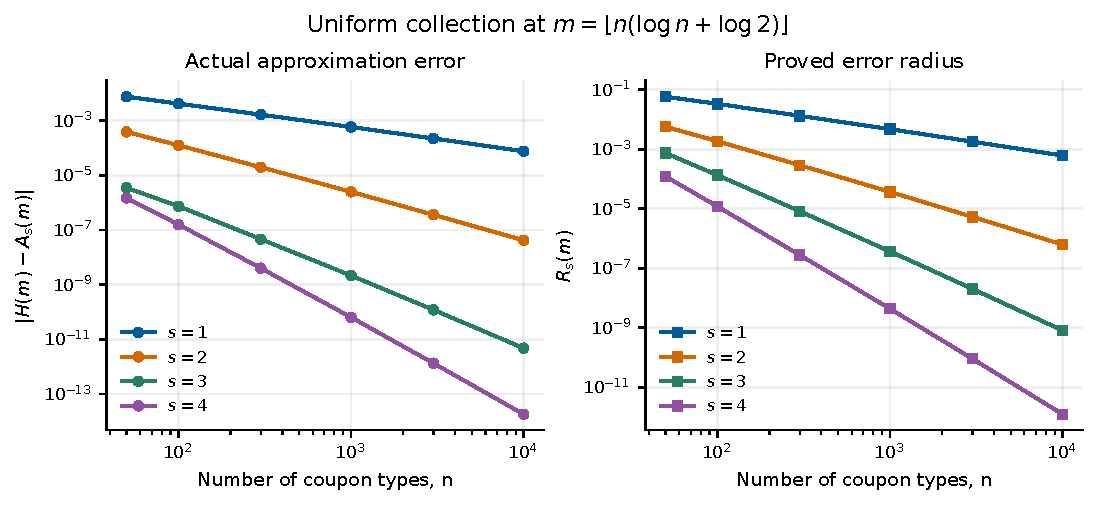
\includegraphics[width=\textwidth]{uniform_errors.pdf}
\caption{Uniform collection in the fixed window $c=\log2$.
The left panel shows the absolute approximation errors; the right panel
shows their certified radii. Points come from the recorded experiments,
with full grouped inclusion--exclusion references. The distinct vertical
scales make the conservatism of a positive radius visible.}
\label{fig:uniform}
\end{figure}

\subsection{Sharpness and unequal probabilities}

The rare-coupon experiment uses $p_1=1/m$, $p_2=1-1/m$ for
$m=10^2,\ldots,10^6$. At $m=10^6$, the ratios
$|P_m-A_s|/R_s$ for $s=1,2,3,4$ are approximately
\[
 0.999999416667,\quad 0.999996833341,\quad
 0.999983208517,\quad 0.999941902368.
\]
These approach one as asserted in \cref{thm:rare}. The smallest radius
in these four cases is about $9.58\cdot10^{-28}$; the reference and
certificate precisions resolve it.

\begin{figure}[H]
\centering
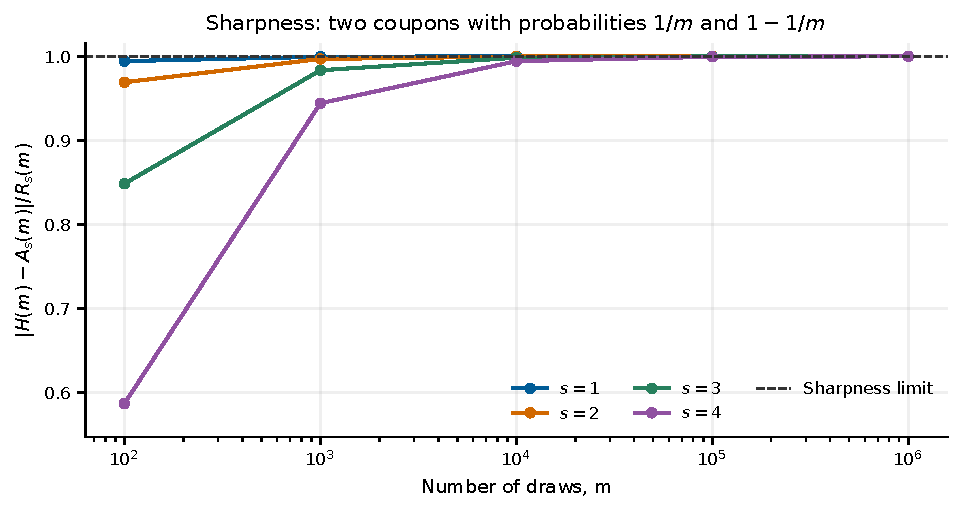
\includegraphics[width=0.88\textwidth]{sharpness_ratio.pdf}
\caption{Asymptotic attainment of the positive radius in the rare-coupon
family. The horizontal line marks ratio one. Each reference is a complete
four-term inclusion--exclusion calculation. The limiting assertion is
\cref{thm:rare}.}
\label{fig:sharpness}
\end{figure}

Two further 100-coupon models test unequal probabilities. The first has
50 coupons of weight one and 50 of weight three. The second has one
coupon of weight one and 99 coupons of weight 100. The weights are
normalized exactly. For each model, three integer times are chosen by
target Poissonized missing means $2$, $0.5$, and $0.05$, and all four
orders are evaluated. The references contain 2601 and 200 grouped terms,
respectively. All reference intervals satisfy containment. The recorded
data retain the exact inputs, achieved missing means, error intervals,
and bound comparisons; the target missing mean is not substituted for
the achieved value in any certificate.

\subsection{Running time and numerical environment}

Timing inputs have $w_i=1+(i\bmod997)$ for $i=0,\ldots,n-1$.
The integer $m$ is chosen so that $\lambda\le0.5$. Equal-weight
grouping is disabled, and timing includes exact normalization and
certificate construction but excludes the selection of $m$.
The implementation used Python 3.12.14, python-flint 0.9.0, one FLINT
thread, and 128-bit arithmetic.

\begin{table}[H]
\centering
\begin{tabular}{@{}rrr@{}}
\toprule
Number of coupons & Order 2 time (s) & Order 3 time (s)\\
\midrule
100 & 0.0036 & 0.0049\\
1000 & 0.0295 & 0.0459\\
10000 & 0.1991 & 0.3450\\
100000 & 2.3039 & 4.0710\\
\bottomrule
\end{tabular}
\caption{One measured run per point after a warm-up. These observations
illustrate the arithmetic scaling; they are not statistical performance
estimates or bit-complexity bounds.}
\label{tab:runtime}
\end{table}

\begin{figure}[H]
\centering
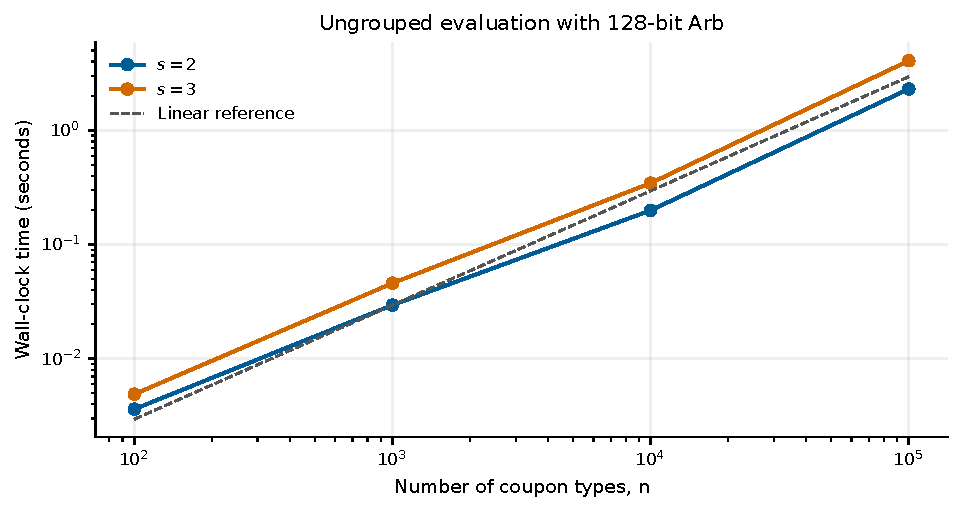
\includegraphics[width=0.88\textwidth]{runtime_scaling.pdf}
\caption{Measured ungrouped evaluation times. The dashed line is
proportional to $n$ and is anchored at the order-two, $n=1000$ measurement.
The proof of \cref{prop:cost} is independent of the timing experiment.}
\label{fig:runtime}
\end{figure}

\section{Consequences and practical interpretation}\label{sec:consequences}

\subsection{From probabilities to sample-size decisions}

A certified probability interval can answer a threshold question:
has the chance of complete coverage reached a chosen target $\alpha$?
If the lower endpoint is at least $\alpha$, the answer is yes. If the
upper endpoint is below $\alpha$, the answer is no. An interval
containing $\alpha$ leaves that particular query unresolved and calls
for a higher order, more arithmetic precision when rounding is relevant,
or a different bound.

Monotonicity of $P_m$ makes it possible to maintain a certified bracket
for the smallest qualifying integer $m$. A binary-search implementation
must preserve that bracket and must not decide from the midpoint of
$A_s$ alone. The approximation $A_s(m)$ itself is not asserted to be
monotone, and no universal exact-quantile complexity follows from this
observation. In particular, a threshold exactly equal to a probability
requires an equality-aware treatment.

\subsection{Why more moments improve a bound}

The strongest part of \eqref{eq:radius} is
\[
 \frac{\binom ms}{2^s}
   \bigl(M_{2s}+sM_{2s+1}+\cdots+M_{3s}\bigr).
\]
Replacing every higher moment by $M_{2s}$ throws away the information
that relevant subset probabilities can be small. When those subsets are
small, $M_{2s+\ell}/M_{2s}$ is small for $\ell>0$, retaining the
factor $2^{-s}$. The rare-coupon family makes this observation exact.
When subset probabilities are not small, the same finite formula remains
valid and records the larger uncertainty.

The mechanism is therefore quantitative rather than heuristic: positivity
of the coefficients gives a global remainder inequality, and the input
moments adapt it to the particular probability vector.

\subsection{An all-orders scalar calculation}

The analytic statement in \cref{thm:optimalsecond} also gives a procedure
for calculating more terms of the optimal constant. Expand
$H_\varepsilon(y)$ from \eqref{eq:scaledlog}; substitute an odd series
$y(\varepsilon)=b_1\varepsilon+b_3\varepsilon^3+\cdots$; solve
$\partial_yH_\varepsilon=0$ successively; and substitute back.
The nonzero coefficient $-2V_s$ makes every step linear in the next
unknown coefficient. All inputs are rational at fixed $s$, so every
coefficient obtained is rational.

This convergent local expansion describes the exact global optimum for
sufficiently large $m$. A finite truncation of that expansion is not
automatically an upper bound: it needs its own explicit remainder before
being used as a numerical certificate. The delivered probability
implementation uses the all-$m$ inequality \eqref{eq:radius}.

\section{Further research questions}\label{sec:future}

The following questions grow directly from proved statements in this
paper. They have different levels of difficulty and should remain
separate from established results.

\begin{enumerate}[label=\textbf{Q\arabic*.},leftmargin=2.7em]
\item \textbf{Explicit finite-$m$ optimal constants.}
Can one bound $\Kopt_{m,s}$ tightly with a small number of operations,
including the range before the asymptotic unique maximum is guaranteed?
A certified one-dimensional optimization could be useful, but an analytic
formula with a verified remainder would be more reusable.

\item \textbf{Growing correction order.}
The proofs keep $s$ fixed. Determine a quantitative range $s=s(m)$ in
which the peak localization, analytic coefficient estimates, and moment
certificate remain effective. This is the step needed for a meaningful
precision-versus-work theorem when the requested number of digits grows
with the input size.

\item \textbf{Cancellation without exponential enumeration.}
The unsigned product loses cancellations between subsets of opposite
parity. Can additional efficiently computable signed information yield
a substantially smaller positive radius, especially for uniform or
nearly uniform inputs? Any such refinement should preserve a complete
error proof.

\item \textbf{Relative error for small coverage probabilities.}
The present radius is additive. Find conditions under which it is at
most $\varepsilon P_m$, or construct a separate factorized certificate
that remains useful before the bounded-$\lambda$ region. Highly unequal
probabilities are the essential test.

\item \textbf{Optimal constants over probability vectors.}
For fixed $L,s$, determine the asymptotic supremum of
$|P_m-A_s|/(\log n/n)^s$ subject to $\lambda\le L$. The Touchard envelope
proves an upper bound, and the uniform family gives nonzero lower
examples, but these constants have not been matched.

\item \textbf{Heterogeneous collection quotas.}
Requiring several copies of each category replaces each Poisson factor
by a Poisson upper-tail probability. Which parts of the positive
coefficient argument survive, and what extra data suffice to certify a
fixed-sample probability efficiently?

\item \textbf{Bit complexity and automatic precision.}
Establish the arithmetic precision needed to make numerical interval
width comparable to the analytic radius for rational inputs of bounded
encoding length. This would convert the present arithmetic count into
a rigorous bit-complexity statement.

\item \textbf{Certified quantiles and sensitivity.}
Combine the intervals with monotonicity and derivative information to
bound coverage-time quantiles and their sensitivity to errors in the
input probabilities. Exact threshold ties and uncertain input
probabilities require explicit treatment.

\item \textbf{Formal verification.}
The finite scalar theorem has a short algebraic structure: coefficient
positivity, a binomial remainder, and a finite signed sum. It is a
plausible first target for a Lean formalization. The analytic maximum
theorem would require a substantially richer formal development.
\end{enumerate}

\appendix
\section{Reproduction and file guide}\label{app:reproduction}

The package contains the LaTeX manuscript and bibliography, the compiled
PDF, the core implementation, an independent test suite, two experiment
programs, recorded data, and the plotting assets. No external manuscript
is bundled as if it were authored here.

From the package directory, install the dependencies and run:
\begin{lstlisting}
python -m pip install -r requirements.txt
python -m unittest discover -s tests -v
python experiments/run_experiments.py
python experiments/sharp_scalar.py
latexmk -pdf -interaction=nonstopmode -halt-on-error \
    -cd article/coupon_collector.tex
\end{lstlisting}
To calculate a single certificate:
\begin{lstlisting}
python src/coupon_certificate.py --uniform 10000 \
    --m 99034 --order 4 --bits 224
python src/coupon_certificate.py --weights 1,2,3,5 \
    --m 100 --order 3 --bits 160
\end{lstlisting}
The experiments record the exact input descriptions, software versions,
working precision, reference method, and a source hash. Timing data are
machine-specific. Re-running the scripts overwrites their generated data
and figures with the new run's measurements.

\begin{longtable}{@{}p{0.39\textwidth}p{0.55\textwidth}@{}}
\toprule
Path & Purpose\\
\midrule
\endhead
\texttt{article/coupon\_collector.tex} & Complete manuscript source.\\
\texttt{article/references.bib} & Primary references and version information.\\
\texttt{src/coupon\_certificate.py} & Rational inputs, product jets, and Arb enclosures.\\
\texttt{tests/test\_certificate.py} & Exact and independent reference checks.\\
\texttt{experiments/run\_experiments.py} & Probability experiments, running times, and figures.\\
\texttt{experiments/sharp\_scalar.py} & Symbolic coefficients and scalar stationary-point checks.\\
\texttt{results/experiments.json} & Full probability and timing records, including ball strings.\\
\texttt{results/*.csv} & Tabular observations for reuse.\\
\texttt{figures/} & PDF and PNG versions of all three figures.\\
\bottomrule
\end{longtable}

\section{A compact checklist of theorem domains}\label{app:domains}

\begin{center}
\small
\begin{tabular}{@{}p{0.28\textwidth}p{0.63\textwidth}@{}}
\toprule
Result & Assumptions and meaning\\
\midrule
\cref{thm:scalar,thm:coupon}
& Positive integers $m,s$; all $x\in[0,1]$ and all probability vectors.
  Finite, explicit absolute-error inequalities.\\[3pt]
\cref{thm:optimalfirst,thm:optimalsecond}
& $s$ fixed, $m\to\infty$ through integers.
  The global maximizer is unique only for sufficiently large $m$.
  The analytic radius in $1/m$ depends on $s$.\\[3pt]
\cref{thm:uniform}
& $s,L$ fixed; $n>L$; $\sum_i e^{-mp_i}\le L$.
  The finite bound is explicit, uniform in $p$ and in every qualifying $m$.\\[3pt]
\cref{thm:rare}
& A distribution varying with $m$.
  The ratio error/radius tends to one for this family.\\[3pt]
\cref{thm:uniformsharp}
& Uniform probabilities and fixed $c$.
  Sharpness concerns the chosen truncation, not every possible algorithm.\\[3pt]
\cref{prop:cost}
& Arithmetic operations and exponential evaluations.
  Extra bit costs and precision requirements are not suppressed as a theorem.\\
\bottomrule
\end{tabular}
\end{center}

\bigskip
The directly strengthened statement is the scalar remainder lemma.
The probability certificate, optimal-constant analysis, sharpness
constructions, and numerical implementation make that improvement
concrete and independently assessable.

\bibliographystyle{plainnat}
\bibliography{references}
\end{document}
